\documentclass{beamer}

% Make nice A4 pages for print:
%\usepackage{pgfpages}
%\pgfpagesuselayout{resize to}[a4paper,border shrink=5mm,landscape]

\beamertemplatenavigationsymbolsempty

\setbeamertemplate{bibliography item}[text]

\usepackage[type={CC},modifier={by-sa},version={4.0}]{doclicense}

\usepackage[utf8]{inputenc}
\usepackage{hyperref}
\usepackage{breakurl}
\usepackage{graphicx}
\usepackage{pgfplots}
\usepackage{pgf}
\usepackage{tikz}
\usetikzlibrary{positioning}
\usetikzlibrary{arrows}
\usetikzlibrary{decorations.markings}
\usetikzlibrary{calc}
\usetikzlibrary{matrix}
\usetikzlibrary{shapes}
\usetikzlibrary{decorations.pathmorphing}
\usetikzlibrary{fit}
\usetikzlibrary{backgrounds}
\usetikzlibrary{plotmarks}
\usepackage{stmaryrd}
\usepackage{listings}
\usepackage{pdflscape}
\usepackage{perpage}
\usepackage{appendixnumberbeamer}

%\usepackage[thmmarks,amsmath,amsthm]{ntheorem} % already included in beamer
\usepackage{thm-restate}

\usepackage[sort&compress,numbers]{natbib}  % to be have \citet, \citeauthor, \citeyear

\MakePerPage{footnote}

\tikzstyle{o}=[r,ppBlue]
\tikzstyle{r}=[thick,rectangle,align=center]
\tikzstyle{t}=[r,ppTrans] %,font=\bfseries]
\tikzstyle{dd}=[densely dashed]
\tikzstyle{n}=[r,ppBlue]
\tikzstyle{p}=[r,ppRed]
\tikzstyle{ppRed}  =[draw=red,  fill=  red!20]
\tikzstyle{ppBlue} =[draw=blue, fill= blue!20]
\tikzstyle{ppGreen}=[draw=green,fill=green!20]
\tikzstyle{ppTrans}=[draw=none, fill=none]

\usetheme{Warsaw}

\useoutertheme[subsection=true]{smoothbars}
%\useoutertheme[subsection=false]{miniframes}

\definecolor{bblue}{HTML}{D7DF01}	% yellow-ish actually, for better black/white printing
\definecolor{rred}{HTML}{C0504D}
\definecolor{ggreen}{HTML}{9BBB59}
\definecolor{ppurple}{HTML}{9F4C7C}
\definecolor{lightgray}{rgb}{0.3,0.3,0.3}
\definecolor{lightergray}{rgb}{0.9,0.9,0.9}
\definecolor{UniBlue}{RGB}{83,121,170}

\DeclareTextFontCommand\textintro{\normalfont\bfseries\itshape} % nice!
\newcommand{\intro}[2][]
{%
	\textintro{#2}%
}
\newcommand{\empha}[2][]
{%
	\emph{#2}%
}

%\theoremstyle{plain}
\newcounter{reqcounter}
\newtheorem{requirement}[reqcounter]{Requirement}

%setbeamercolor{structure}{fg=violet}

\makeatletter
\def\th@task{%
    \normalfont % body font
    \setbeamercolor{block title example}{bg=orange,fg=white}
    \setbeamercolor{block body example}{bg=orange!20,fg=black}
    \def\inserttheoremblockenv{exampleblock}
  }
\makeatother

\theoremstyle{task}
\newtheorem{task}{Task}

\newenvironment{assignment}%
{%\setbeamercolor{background canvas}{bg=violet}%
%\setbeamercolor{structure}{fg=cyan!90!black}%
 \setbeamercolor{frametitle}{bg=orange,fg=white}
\begin{frame}}%
{\end{frame}}%

\AtBeginSection[]{
  \begin{frame}
  \vfill
  \centering
  \begin{beamercolorbox}[sep=8pt,center,shadow=true,rounded=true]{title}
    \usebeamerfont{title}\insertsectionhead\par%
  \end{beamercolorbox}
  \tableofcontents
  \vfill
  \end{frame}
}




\pgfplotsset{compat=1.14}
\author{Markus Raab}


\date{9.3.2018}

\begin{document}

\renewcommand{\enquote}[1]{\emph{``#1''}} % Cannot be done earlier

%%%%%%%%%%%%%%%%%%%%%%%%%%%%%%%
\begin{frame}
	\titlepage
	\doclicenseThis
\end{frame}

\begin{assignment}
	\frametitle{Language of the Talk?}
	\begin{task}
	Hands up if you prefer German.
	\end{task}
	Unanimous preference of German required, otherwise English.
\end{assignment}

\begin{frame}
	\frametitle{Organization}
	\begin{description}
		\item[20.4.2018:] no lecture
	\end{description}
\end{frame}

\section{Configuration File Formats}

\subsection{Definitions}

\begin{frame}
	\frametitle{Basic Definitions}
	The \intro[execution environment]{execution environment} is information outside the boundaries of each currently running process~\cite{corbato1971multics}.

	Controlling the execution environment is essential for configuration management~\cite{cons2002pan,huang2015confvalley}, testing~\cite{van2010automating,wang2009context}, and security~\cite{goldberg1996secure,schreuders2012towards,perkins2009automatically,liang2003isolated}.
\end{frame}

\begin{frame}
	\frametitle{Configuration Setting}
	\begin{definition}
\label{def:configuration-setting}
A \intro[configuration setting]{configuration setting},
or \intro[setting|see{configuration setting}]{setting} in short,
fulfills these properties:
\begin{enumerate}
\item
It is provided by the execution environment.
\item
It is \empha[consume]{consumed} by an application.
\item
It consists of a key, a configuration value, and potentially \empha{metadata}.
The \intro{configuration value}, or \intro[value|see{configuration value}]{value} in short, influences the application's behavior.
\item
It can be \empha[produce]{produced} by the maintainer, user, or system administrator of the software.
\end{enumerate}
\end{definition}

\end{frame}


\begin{frame}[fragile]
	\frametitle{Synonyms}
\intro[user preferences|see{configuration setting}]{User preferences}~\cite{jin2014configurations} and \intro[customization|see{configuration setting}]{customization}~\cite{anderson2002researching} stress that users make the change although that might not always be the case.
\intro[variability point|see{configuration setting}]{Variability points}~\cite{gunther2012software,rhein2016variability,villela2014survey,van2001notion,nadi2014mining,mens2016taxonomy} aim at describing the capability of software to adapt its behavior.
\intro[derivation decision|see{configuration setting}]{Derivation decision}~\cite{software1993reuse,czarnecki2012cool} puts the decisions to make and not the result in focus.
\intro[configuration parameter|see{configuration setting}]{Configuration parameter}~\cite{yin2011empirical,anderson1994towards} is easily confused with other kinds of parameters.
\intro[configuration item|see{configuration setting}]{Configuration item}~\cite{anthony2009context} or \intro[configuration option|see{configuration setting}]{configuration option}~\cite{rabkin2011static,zhang2013automated,zhang2014configuration} are sometimes not applicable, for example, ``proxy option'', or ``language item''.
\intro[configuration data|see{configuration setting}]{Configuration data}~\cite{huang2015confvalley} is often used in the context of programmable gate arrays and has a different meaning in that domain.
\end{frame}

\begin{frame}[fragile]
	\frametitle{Definition}
	A \intro{configuration file} is a file containing configuration settings.

	\pause
	A Web server configuration file:

\begin{lstlisting}
port=80 ; comment
address=127.0.0.1\end{lstlisting}

	\only<2-2>{
	\begin{task}
	What are keys? What are configuration values? What is metadata?
	\end{task}
	}
	\pause

	The configuration values are ^80^ and ^127.0.0.1^, respectively.
	Other information in the configuration file is metadata for the configuration settings (such as the comment).
\end{frame}

\subsection{Formats}

\begin{frame}
	\frametitle{}
\end{frame}

\begin{frame}
	\frametitle{CSV formats}
	\begin{itemize}
	\item e.g., passwd, group (:)
	\item are difficult to extend (e.g., GECOS)
	\item only used for legacy reasons
	\end{itemize}
\end{frame}

\begin{frame}
	\frametitle{Trends}
	\begin{itemize}
	\item away from CSV
	\item general-purpose serialization formats
	\item human-read/writable (YAML, HOCON, TOML)
	\item programming language as configuration file (e.g., for window managers)
	\end{itemize}
\end{frame}

\begin{assignment}
	\frametitle{Introduce somebody}
	\begin{task}
	Talk with someone else about your favourite configuration file format.
	\end{task}

	\begin{task}
	Explain to everyone about the other person and the favourite configuration file format.
	\end{task}
\end{assignment}

\subsection{Requirements}
\subsection{Abstractions}

\begin{frame}
	\frametitle{Key-Value}
A key-value pair is the simplest generic data structure~\cite{strang2004context}.
While all these formats above have many differences, all of them represent configuration settings as \intro[key-value pair]{key-value pairs}~\cite{jin2014configurations,rabkin2011static,xu2013blame,lathia2013open}.
\end{frame}

\begin{frame}
	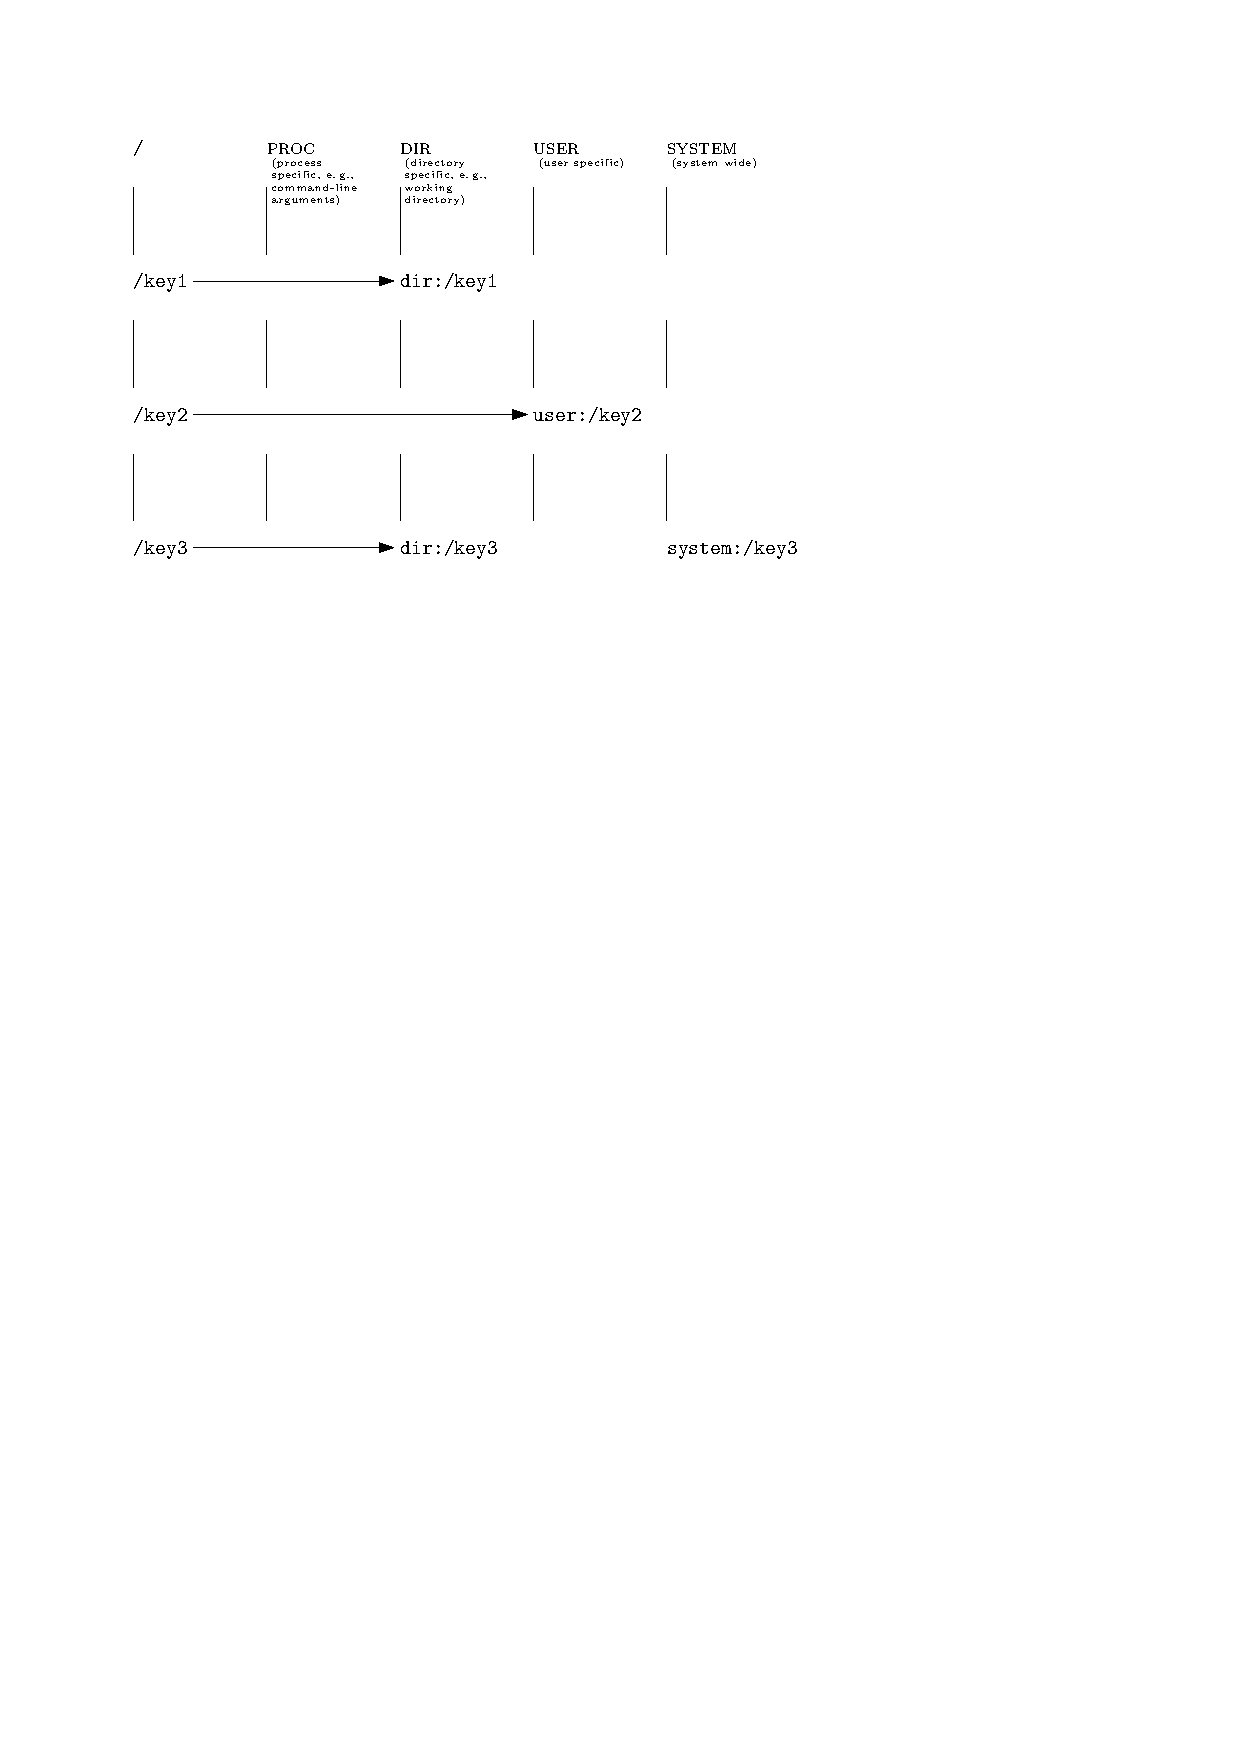
\includegraphics{cascading}
\end{frame}

\begin{frame}
	\frametitle{Mounting}
	\intro[mounting]{Mounting} integrates a backend into the key database~\cite{raab2008thesis}.
	Hence, \elektra{} allows several backends to deal with configuration files at the same time.
	Each backend is responsible for its own subtree of the key database.

	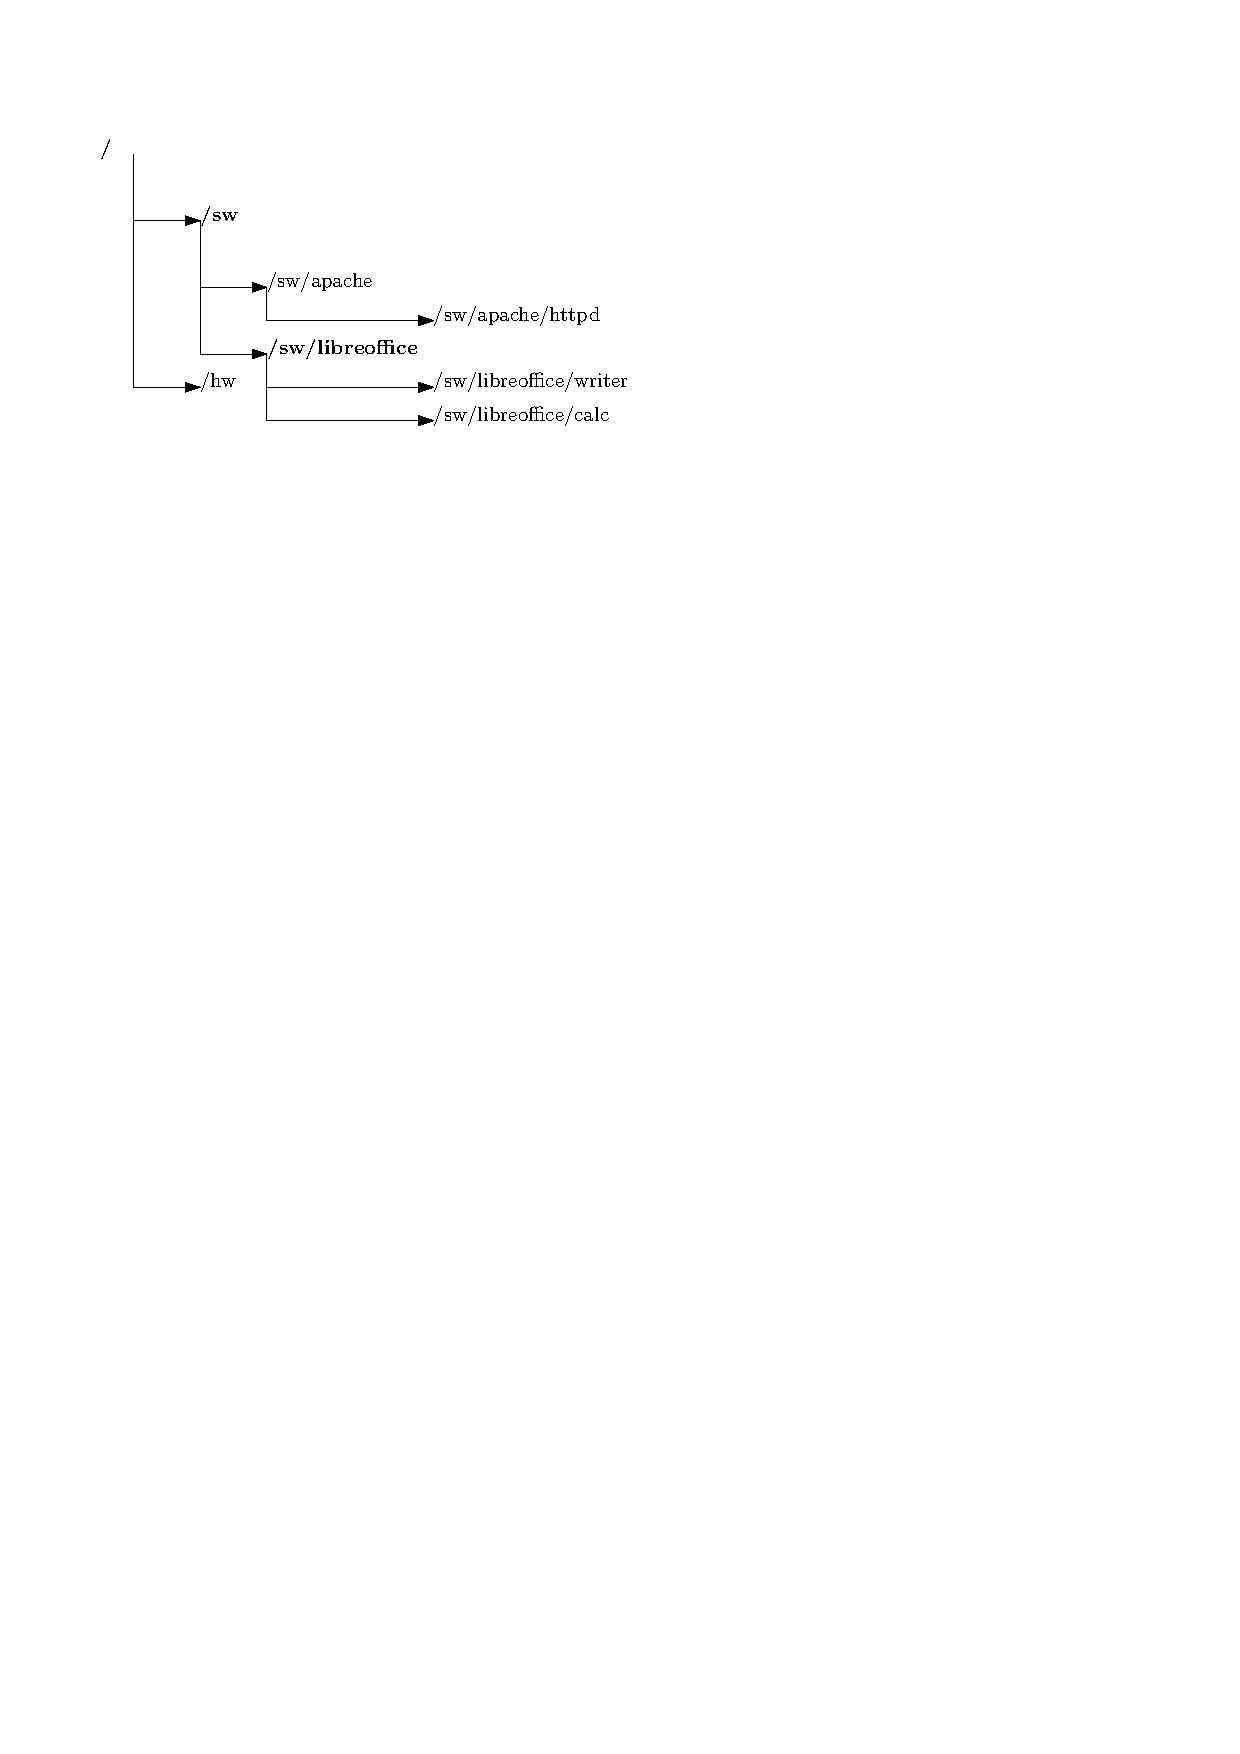
\includegraphics{mounting}
\end{frame}

\begin{frame}
	\frametitle{Plugins}
\end{frame}

\begin{assignment}
	\begin{task}
	Possible Task: Implement a storage plugin with existing parser.
	\end{task}

	\begin{task}
	Discuss the differences of cascading, mounting, and plugins with your neighbor.
	\end{task}
\end{assignment}

\section{Command-line Arguments}
\section{Environment Variables}

\begin{frame}
	\frametitle{Portability}
	\begin{itemize}
	\item separators
	\item case sensitivity
	\end{itemize}
\end{frame}



%%%%%%%%%%%%%%%%%%%%%%%%%%%%%%%%%%%%%%%%%% 
\nocite{raab2017introducing}

\appendix

\begin{frame}[allowframebreaks]
	\bibliographystyle{plainnat}
	\bibliography{../shared/elektra.bib}
\end{frame}

\end{document}


